\documentclass[t,usenames,dvipsnames]{beamer}
\usetheme{Copenhagen}
\setbeamertemplate{headline}{} % remove toc from headers
\beamertemplatenavigationsymbolsempty

\usepackage{amsmath, tikz, xcolor, array, pgf, pgfplots}
\pgfplotsset{compat=newest}
\usetikzlibrary{arrows.meta}
\everymath{\displaystyle}
\tikzset{>=stealth}

\title{Linear Functions and Slope}
\author{}
\date{}

\AtBeginSection[]
{
  \begin{frame}
    \frametitle{Objectives}
    \tableofcontents[currentsection]
  \end{frame}
}

\begin{document}

\begin{frame}
    \titlepage
\end{frame}

\section{Calculate the slope of a line connecting two points}

\begin{frame}{Slope}
    The slope of the line connect points $P(x_1,y_1)$ and $Q(x_2,y_2)$ is
    \[ m = \frac{y_2-y_1}{x_2-x_1} \]
    provided $x_2 \neq x_1$
\end{frame}

\begin{frame}{Example 1}
Find the slope of the line connecting each pair of points. \newline\\
(a) \quad $(0,0)$ and $(2,4)$   \newline\\
\begin{minipage}{0.5\textwidth}
\begin{tikzpicture}[scale=0.7]
\draw[->] (-1,0)--(5,0) node [right] {$x$};
\draw[->] (0,-1) -- (0,5) node [above] {$y$};
\foreach \x in {1,2,3,4}
\draw (\x, 0.1) -- (\x, -0.1) node [below] {\scriptsize $\x$};
\foreach \y in {1,2,3,4}
\draw (0.1,\y) -- (-0.1,\y) node [left] {\scriptsize $\y$};
\draw[color=red,fill=red] (0,0) circle (2pt);
\draw[color=red,fill=red] (2,4) circle (2pt);
\draw[<->,color=red,thick,domain=-0.25:2.25] plot ({\x,2*\x});
\end{tikzpicture}
\end{minipage}
\hspace{0.25cm}
\begin{minipage}{0.35\textwidth}
\begin{align*}
    \onslide<2->{m &= \frac{y_2-y_1}{x_2-x_1}} \\[10pt]
    \onslide<3->{&= \frac{4-0}{2-0}} \\[10pt]
    \onslide<4->{&= 2}
\end{align*}
\end{minipage}
\end{frame}


\begin{frame}{Example 1}
(b) \quad $(-2,3)$ and $(2,-3)$   \newline\\
\begin{minipage}{0.5\textwidth}
\begin{tikzpicture}[scale=0.65]
\draw[<->] (-3.5,0)--(4,0) node [right] {$x$};
\draw[<->] (0,-4.5) -- (0,4.5) node [above] {$y$};
\foreach \x in {-3,-2,-1,,1,2,3}
\draw (\x, 0.1) -- (\x, -0.1) node [below] {\scriptsize $\x$};
\foreach \y in {-4,-3,-2,-1,,1,2,3,4}
\draw (0.1,\y) -- (-0.1,\y) node [left] {\scriptsize $\y$};
\draw[color=red,fill=red] (-2,3) circle (2pt);
\draw[color=red,fill=red] (2,-3) circle (2pt);
\draw[<->,color=red,thick,domain=-2.75:2.75] plot ({\x,-1.5*\x});
\end{tikzpicture}
\end{minipage}
\hspace{0.25cm}
\begin{minipage}{0.35\textwidth}
\begin{align*}
    \onslide<2->{m &= \frac{y_2-y_1}{x_2-x_1}} \\[10pt]
    \onslide<3->{&= \frac{-3-3}{2-(-2)}} \\[10pt]
    \onslide<4->{&= \frac{-6}{4}} \\[10pt]
    \onslide<5->{&= -\frac{3}{2}}
\end{align*}
\end{minipage}
\end{frame}


\begin{frame}{Example 1}
(c) \quad $(-3,2)$ and $(4,2)$   \newline\\
\begin{minipage}{0.5\textwidth}
\begin{tikzpicture}[scale=0.65]
\draw[<->] (-4.5,0)--(4.5,0) node [right] {$x$};
\draw[->] (0,0) -- (0,3.5) node [above] {$y$};
\foreach \x in {-4,-3,-2,-1,,1,2,3,4}
\draw (\x, 0.1) -- (\x, -0.1) node [below] {\scriptsize $\x$};
\foreach \y in {1,2,3}
\draw (0.1,\y) -- (-0.1,\y) node [left] {\scriptsize $\y$};
\draw[color=red,fill=red] (-3,2) circle (2pt);
\draw[color=red,fill=red] (4,2) circle (2pt);
\draw[<->,color=red,thick] (-4,2) -- (4.5,2);
\end{tikzpicture}
\end{minipage}
\hspace{0.25cm}
\begin{minipage}{0.35\textwidth}
\begin{align*}
    \onslide<2->{m &= \frac{y_2-y_1}{x_2-x_1}} \\[10pt]
    \onslide<3->{&= \frac{2-2}{4-(-3)}} \\[10pt]
    \onslide<4->{&= \frac{0}{7}} \\[10pt]
    \onslide<5->{&= 0}
\end{align*}
\end{minipage}
\end{frame}


\begin{frame}{Example 1}
(d) \quad $(2,3)$ and $(2,-1)$   \newline\\
\begin{minipage}{0.5\textwidth}
\begin{tikzpicture}[scale=0.65]
\draw[->] (0,0)--(3,0) node [right] {$x$};
\draw[->] (0,-4) -- (0,4) node [above] {$y$};
\foreach \x in {1,2}
\draw (\x, 0.1) -- (\x, -0.1) node [below] {\scriptsize $\x$};
\foreach \y in {-3,-2,-1,,1,2,3}
\draw (0.1,\y) -- (-0.1,\y) node [left] {\scriptsize $\y$};
\draw[color=red,fill=red] (2,3) circle (2pt);
\draw[color=red,fill=red] (2,-1) circle (2pt);
\draw[<->,color=red,thick] (2,-4) -- (2,4);
\end{tikzpicture}
\end{minipage}
\hspace{0.25cm}
\begin{minipage}{0.35\textwidth}
\begin{align*}
    \onslide<2->{m &= \frac{y_2-y_1}{x_2-x_1}} \\[10pt]
    \onslide<3->{&= \frac{-1-3}{2-2}} \\[10pt]
    \onslide<4->{&= \frac{-4}{0}} \\[10pt]
    \onslide<5->{&= \text{undefined}}
\end{align*}
\end{minipage}
\end{frame}

\section{Write the point-slope form of a line}

\begin{frame}{Point-Slope Form of a Line}

The \alert{point-slope form} of a line is a general equation involving the slope of the line and a point on the line.
    \begin{align*}
        \onslide<2->{m &= \frac{y-y_1}{x-x_1}} \\[10pt]
        \onslide<3->{m(x-x_1) &= y - y_1} \\[10pt]
        \onslide<4->{y-y_1 &= m(x-x_1)}
    \end{align*}
\end{frame}

\begin{frame}{Example 2}
Write the equation of the line connecting the points $(-1,3)$ and $(2,1)$.
\begin{align*}
    \onslide<2->{m &= \frac{1-3}{2-(-1)}} \\[8pt]
    \onslide<3->{m &= -\frac{2}{3}} \\[8pt]
    \onslide<4->{y-3 &= -\frac{2}{3}\left(x-(-1)\right)} \\[8pt]
    \onslide<5->{y-3 &= -\frac{2}{3}\left(x+1\right)}
\end{align*}
\end{frame}

\section{Write the equation of a line in slope-intercept form}

\begin{frame}{Slope-Intercept Form}
The \alert{slope-intercept form} of the equation of a line is
\[ y = mx + b \]
where $b$ is the $y$-intercept. \newline\\ \pause

To convert from point-slope form to slope-intercept form, solve the point-slope form for $y$.
\end{frame}

\begin{frame}{Example 3}
Convert $y-3 = -\dfrac{2}{3}\left(x+1\right)$ to slope-intercept form.
\begin{align*}
    \onslide<2->{y-3 &= -\frac{2}{3}\left(x+1\right)} \\[8pt]
    \onslide<3->{y-3 &= -\frac{2}{3}x - \frac{2}{3}} \\[8pt]
    \onslide<4->{y &= -\frac{2}{3}x + \frac{7}{3}}
\end{align*}
\end{frame}

\section{Determine the average rate of change of a function}

\begin{frame}{Average Rate of Change}
The \alert{average rate of change} over an interval $[a,b]$ of a function is the slope of the line connecting the endpoints of the interval.  \pause
\[
\frac{\Delta f}{\Delta x} = \frac{f(b)-f(a)}{b-a}
\]
\end{frame}

\begin{frame}{Average Rate of Change}
\begin{center}
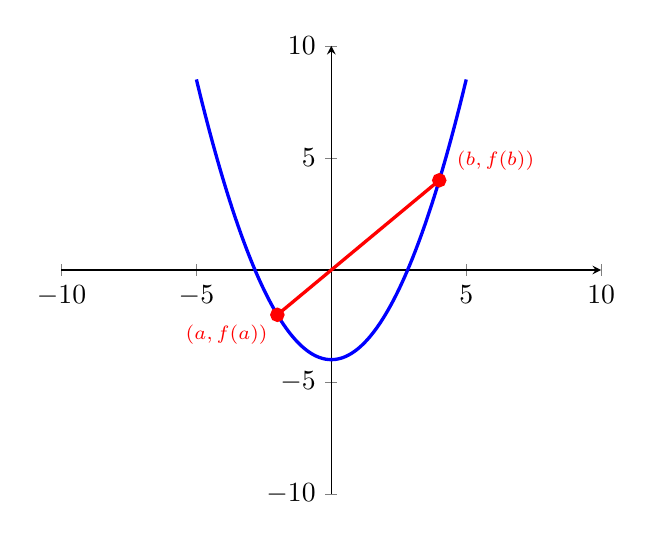
\begin{tikzpicture}
\begin{axis}[
axis lines = middle,
xmin = -10, xmax = 10,
ymin = -10, ymax = 10,
]
\addplot[blue,very thick,samples=200,smooth] {0.5*x^2-4};
\addplot[mark=*, red, very thick] coordinates {(-2,-2) (4,4)};
\node at (axis cs: -2,-2) [below left, red] {\scriptsize $(a,f(a))$};
\node at (axis cs: 4,4) [above right, red, xshift=0.1cm] {\scriptsize $(b,f(b))$};
\end{axis}
\end{tikzpicture}
\end{center}
\end{frame}

\begin{frame}{Example 4}
Find the average rate of change for each.   \newline\\
(a) \quad $f(x) = \dfrac{1}{x} \quad [1,5]$  \newline\\
\begin{minipage}{0.55\textwidth}
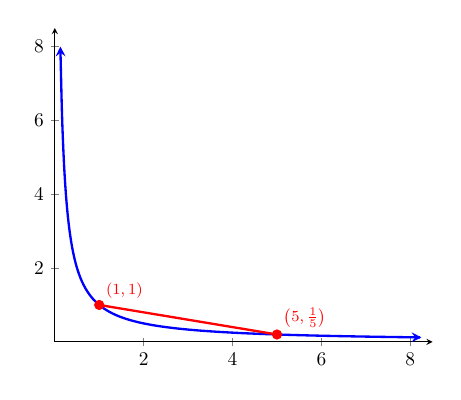
\begin{tikzpicture}[scale=0.7]
\begin{axis}[
axis lines = center,
xmin = 0, xmax = 8.5,
ymin = 0, ymax = 8.5,
]
\addplot[<->,blue,very thick,domain=0.125:8.25, samples=200, smooth] {1/x};
\addplot[color=red,very thick, mark = *] coordinates {(1,1) (5,0.2)};
\node at (axis cs: 1,1) [above right, color=red] {\footnotesize $(1,1)$}; 
\node at (axis cs: 5,0.2) [above right, color=red] {\footnotesize $\left(5,\frac{1}{5}\right)$};
\end{axis}
\end{tikzpicture}
\end{minipage}
\hspace{-0.25cm}
\begin{minipage}{0.35\textwidth}
\begin{align*}
    \onslide<2->{f(5) &= \frac{1}{5} & f(1) &= 1} \\[10pt]
    \onslide<3->{&\frac{\Delta f}{\Delta x} &= \frac{\frac{1}{5}-1}{5-1}\left(\frac{5}{5}\right)&}
    \\[10pt]
    \onslide<4->{&\frac{\Delta f}{\Delta x} &= \frac{1-5}{25-5}&} \\[10pt]
    \onslide<5->{&&=-\frac{1}{5}&}
\end{align*}
\end{minipage}
\end{frame}


\begin{frame}{Example 4}
(b) \quad $f(x) = 3x^2 + 2x - 7 \qquad [-2, 2]$ \newline\\
\begin{minipage}{0.55\textwidth}
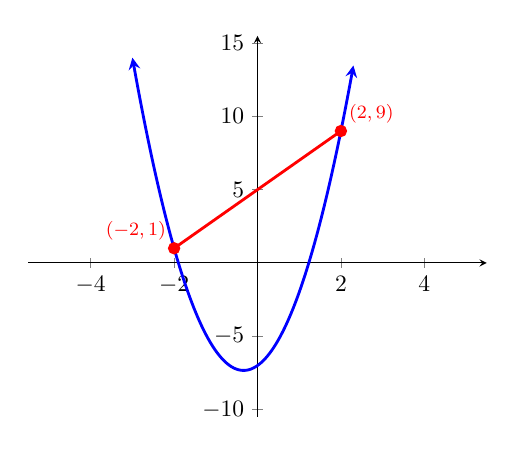
\begin{tikzpicture}[scale=0.85]
\begin{axis}[
axis lines = center,
xmin = -5.5, xmax = 5.5,
ymin = -10.5, ymax = 15.5,
]
\addplot[<->,blue,very thick,domain=-3:2.3, samples=200, smooth] {3*x^2+2*x-7};
\addplot[color=red,very thick, mark = *] coordinates {(-2,1) (2,9)};
\node at (axis cs: -2,1) [above left, color=red] {\footnotesize $(-2,1)$}; 
\node at (axis cs: 2,9) [above right, color=red] {\footnotesize $(2,9)$};
\end{axis}
\end{tikzpicture}
\end{minipage}
\hspace{-0.25cm}
\begin{minipage}{0.35\textwidth}
\begin{align*}
    \onslide<2->{f(2) &= 9 & f(-2) &= 1} \\[12pt]
    \onslide<3->{&\frac{\Delta f}{\Delta x} &= \frac{9-1}{2-(-2)}&}
    \\[12pt]
    \onslide<4->{&\frac{\Delta f}{\Delta x} &= \frac{8}{4}&} \\[12pt]
    \onslide<5->{&&=2&}
\end{align*}
\end{minipage}
\end{frame}

\section{Find the least-squares regression line}

\begin{frame}{Least-Squares Regression Line}
When we plot data points, we can sometimes create a least squares regression line to describe and predict the data.   \newline\\

The value of $r$ (the correlation coefficient) determines how well the data ``falls into line." \newline\\

The closer $r$ is to 1 (or $-1$) the better the linear fit.
\end{frame}

\begin{frame}{Example 5}
    The census data for Lake County, Ohio is shown: \newline\\
    \begin{center}
        \begin{tabular}{|c|c|c|c|c|c|}
        \hline
            \textbf{Year} & 1970 & 1980 & 1990 & 2000 & 2010 \\ \hline
            \textbf{Pop} & 197200 & 212801 & 215499 & 227511 & 230041 \\ 
        \hline
        \end{tabular}   \newline\\
    \end{center}
    (a) Find the least-squares regression line. \pause
    \[  y = 803.92x + 200532 \] \pause
    (b) Interpret the slope. \pause \newline\\
    Population increases by about 804 people per year.
\end{frame}

\begin{frame}{Example 5}
\[  y = 803.92x + 200532 \]
(c) Predict the population of Lake County in 2070.   \pause
\[ 803.92(100) + 200532 = 280924 \] \pause
(d) In what year is the population predicted to exceed 250,000? 
\begin{align*}
    \onslide<4->{802.92x + 200532 &> 250000}    \\
    \onslide<5->{x &> 61.5} \\
\end{align*}
\onslide<6->{Predicted to exceed 250,000 in the year 2031.}
\end{frame}

\end{document}
